\documentclass[12pt]{article}

\usepackage[T1]{fontenc}
\usepackage{graphicx}
\graphicspath{ {./images/} } 
\usepackage{float}
\begin{document}

(Q)
Describe: ...
\clearpage

SCC361: Artificial Intelligence\\
Week 1: Introduction to Artificial Intelligence and Machine Learning\\
Dr Bryan M. Williams\\
School of Computing and Communications, Lancaster University\\
Office: InfoLab21 C40 Email: b.williams6@lancaster.ac.uk\\
1\\
\begin{figure}[H]

\includegraphics[width=0.5\linewidth]{page1-image-1.png}
\end{figure}
\clearpage
(Q)
Describe: SCC361: Artificial Intelligence
\clearpage
\section{SCC361: Artificial Intelligence}
\\
2\\
Lectures, Materials and Expectations\\
Introduction to the Module\\
Overview of Artificial Intelligence\\
Overview of Machine Learning\\
\begin{figure}[H]

\includegraphics[width=0.5\linewidth]{page1-image-1.png}
\end{figure}
\begin{figure}[H]

\includegraphics[width=0.5\linewidth]{page1-image-2.png}
\end{figure}
\begin{figure}[H]
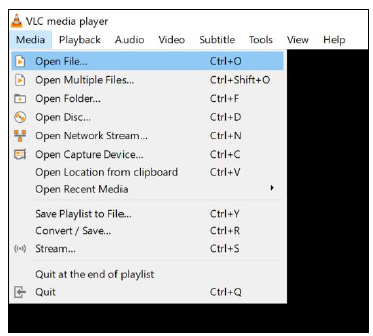
\includegraphics[width=0.5\linewidth]{page1-image-3.png}
\end{figure}
\begin{figure}[H]
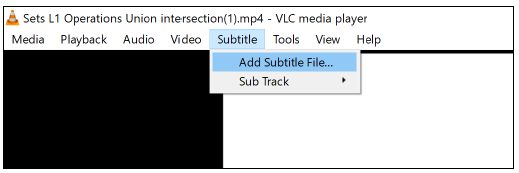
\includegraphics[width=0.5\linewidth]{page1-image-4.png}
\end{figure}
\begin{figure}[H]

\includegraphics[width=0.5\linewidth]{page1-image-5.png}
\end{figure}
\begin{figure}[H]

\includegraphics[width=0.5\linewidth]{page1-image-6.png}
\end{figure}
\begin{figure}[H]

\includegraphics[width=0.5\linewidth]{page1-image-7.png}
\end{figure}
\begin{figure}[H]

\includegraphics[width=0.5\linewidth]{page1-image-8.png}
\end{figure}
\begin{figure}[H]

\includegraphics[width=0.5\linewidth]{page1-image-9.png}
\end{figure}
\begin{figure}[H]

\includegraphics[width=0.5\linewidth]{page1-image-10.png}
\end{figure}
\clearpage
(Q)
Describe: Playing this Video
\clearpage
\section{Playing this Video}
\\
\begin{itemize}
  \item This version is unedited
  \item In general, it might be slow for some people
  \item Vary the playback speed to suit you preferred pace
  \item In live sessions, you can ask questions at any stage, but the 
\end{itemize}
Questions? slides will give you a specific opportunity to ask \\
questions\\
\begin{itemize}
  \item While watching, use the Questions? slides as stop points for 
\end{itemize}
coffee breaks, notes etc\\
3\\
\begin{figure}[H]

\includegraphics[width=0.5\linewidth]{page1-image-1.png}
\end{figure}
\begin{figure}[H]

\includegraphics[width=0.5\linewidth]{page1-image-2.png}
\end{figure}
\begin{figure}[H]
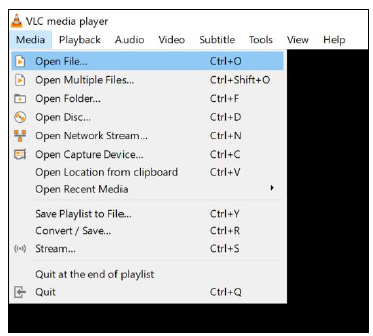
\includegraphics[width=0.5\linewidth]{page1-image-3.png}
\end{figure}
\clearpage
(Q)
Describe: Accessibility
\clearpage
\section{Accessibility}
\\
\begin{itemize}
  \item All our content is expected to meet the UK 
\end{itemize}
accessibility requirements\\
\begin{itemize}
  \item We have done our best to ensure that that is the 
\end{itemize}
case with these course materials\\
\begin{itemize}
  \item However, if any course material or part of its content 
\end{itemize}
is inaccessible in anyway to any individual or group, \\
kindly let us know.\\
4\\
\begin{figure}[H]

\includegraphics[width=0.5\linewidth]{page1-image-1.png}
\end{figure}
\begin{figure}[H]

\includegraphics[width=0.5\linewidth]{page1-image-2.png}
\end{figure}
\begin{figure}[H]
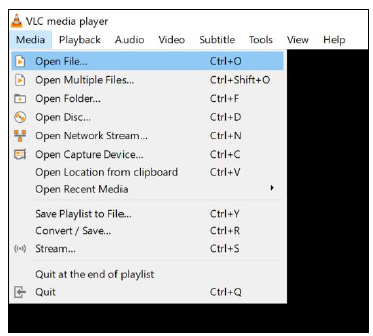
\includegraphics[width=0.5\linewidth]{page1-image-3.png}
\end{figure}
\clearpage
(Q)
Describe: Be sure to check in to all timetabled sessions using 
\clearpage
\section{Be sure to check in to all timetabled sessions using }
\\
Attendance Check-in\\
To check in:\\
\begin{itemize}
  \item Check the Attendance Hub in iLancaster
  \item Click Check In
  \item Wait for the “You are checked in” confirmation page
  \item Here is a the demo
\end{itemize}
Please DO NOT leave a timetabled session without your\\
attendance being registered\\
Attendance Check-in\\
5\\
\begin{figure}[H]

\includegraphics[width=0.5\linewidth]{page1-image-1.png}
\end{figure}
\begin{figure}[H]

\includegraphics[width=0.5\linewidth]{page1-image-2.png}
\end{figure}
\begin{figure}[H]
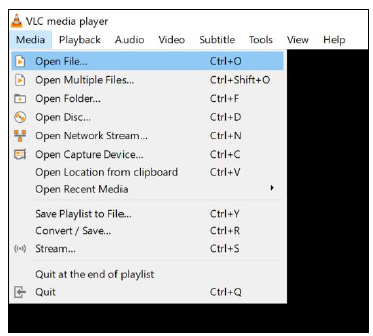
\includegraphics[width=0.5\linewidth]{page1-image-3.png}
\end{figure}
\clearpage
(Q)
Describe: Online Sessions on Teams
\clearpage
\section{Online Sessions on Teams}
\\
Before the session:\\
\begin{itemize}
  \item Follow the Moodle link to join the lecture
  \item Ensure that your speakers, headsets are connected and working
\end{itemize}
6\\
\begin{figure}[H]

\includegraphics[width=0.5\linewidth]{page1-image-1.png}
\end{figure}
\begin{figure}[H]

\includegraphics[width=0.5\linewidth]{page1-image-2.png}
\end{figure}
\begin{figure}[H]
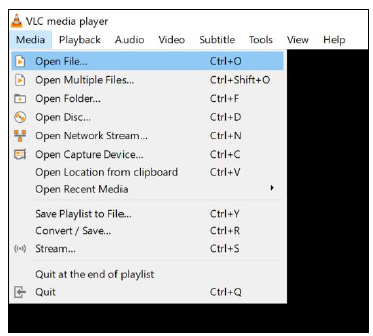
\includegraphics[width=0.5\linewidth]{page1-image-3.png}
\end{figure}
\clearpage
(Q)
Describe: Online Sessions on Teams
\clearpage
\section{Online Sessions on Teams}
\\
During the lectures:\\
\begin{itemize}
  \item Turn your webcam off
  \item Turn your microphone off
\end{itemize}
7\\
\begin{figure}[H]

\includegraphics[width=0.5\linewidth]{page1-image-1.png}
\end{figure}
\begin{figure}[H]

\includegraphics[width=0.5\linewidth]{page1-image-2.png}
\end{figure}
\begin{figure}[H]
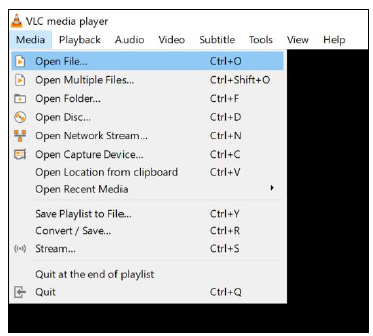
\includegraphics[width=0.5\linewidth]{page1-image-3.png}
\end{figure}
\clearpage
(Q)
Describe: Online Sessions on Teams
\clearpage
\section{Online Sessions on Teams}
\\
During the lectures:\\
\begin{itemize}
  \item Use  chat  appropriately. Not closely monitored during lectures.
\end{itemize}
For live Q\&A sessions:\\
\begin{itemize}
  \item Raise your hand to ask questions. Lower it afterwards.
  \item When called, turn on your mic (and cam if you wish). Remember to turn them off 
\end{itemize}
afterwards.\\
Post additional questions on the SCC361 Moodle Forum\\
8\\
\begin{figure}[H]

\includegraphics[width=0.5\linewidth]{page1-image-1.png}
\end{figure}
\begin{figure}[H]

\includegraphics[width=0.5\linewidth]{page1-image-2.png}
\end{figure}
\begin{figure}[H]
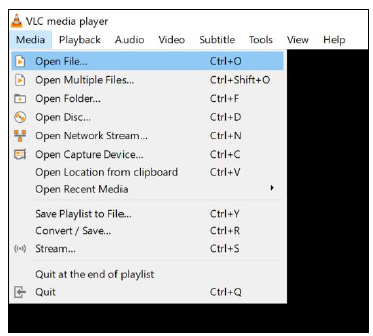
\includegraphics[width=0.5\linewidth]{page1-image-3.png}
\end{figure}
\clearpage
(Q)
Describe: Online Sessions on Teams
\clearpage
\section{Online Sessions on Teams}
\\
After the lectures:\\
\begin{itemize}
  \item The recorded content of the live sessions will be made available after the session on the 
\end{itemize}
Moodle Space\\
9\\
\begin{figure}[H]

\includegraphics[width=0.5\linewidth]{page1-image-1.png}
\end{figure}
\begin{figure}[H]

\includegraphics[width=0.5\linewidth]{page1-image-2.png}
\end{figure}
\begin{figure}[H]
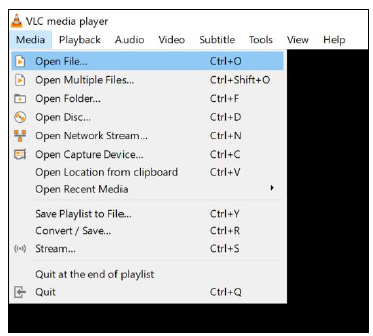
\includegraphics[width=0.5\linewidth]{page1-image-3.png}
\end{figure}
\clearpage
(Q)
Describe: The lectures can be watched on the Moodle space.
\clearpage
\section{The lectures can be watched on the Moodle space.}
\\
If you are struggling to watch the videos on Moodle:\\
\begin{itemize}
  \item Download the video and caption file (*.vtt) from Moodle
  \item Download the free, open source VLC Media player: 
\end{itemize}
https://www.videolan.org/vlc/index.en-GB.html\\
\begin{itemize}
  \item Open video file in VLC and add caption file
\end{itemize}
Note:\\
All learning materials: slides, videos and caption\\
files are @Lancaster University copyright and are \\
not to be shared or distributed.\\
Using Materials Offline\\
10\\
\begin{figure}[H]

\includegraphics[width=0.5\linewidth]{page1-image-1.png}
\end{figure}
\begin{figure}[H]

\includegraphics[width=0.5\linewidth]{page1-image-2.png}
\end{figure}
\begin{figure}[H]
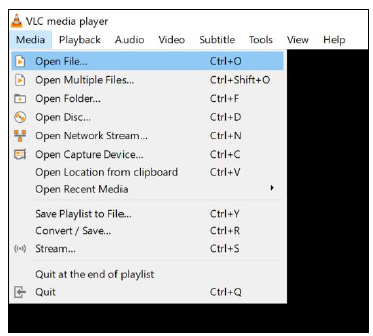
\includegraphics[width=0.5\linewidth]{page1-image-3.png}
\end{figure}
\begin{figure}[H]
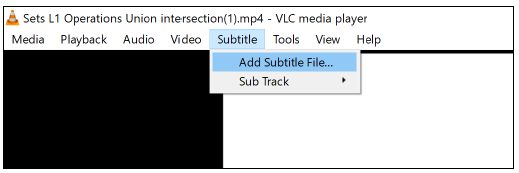
\includegraphics[width=0.5\linewidth]{page1-image-4.png}
\end{figure}
\clearpage
(Q)
Describe: ...
\clearpage
\clearpage
(Q)
Describe: ...
\clearpage
\\
\end{document}